%% Lecture 06
\section{Geometric Multigrid}

A popular iterative method for numerically solving differential equations
is knows as the \emph{Multigrid Method}. We build up to the method by first
exploring a variety of simpler methods. Many of the notes from this section are
from the book by \cite{briggs-2000}. 

\subsection{Finite Difference for Elliptic PDEs}

Consider the BVP

\begin{align*}
-&u^{''}(x) + \sigma u(x) = f(x) \qquad x\in (0,1),\, \sigma \geq 0 \\
 &u(0)=u(1)=0
\end{align*}

Diseretize at the $n$ interior points

\begin{equation*}
x_i = ih, \quad i=1, \ldots, n \quad \text{and} \quad h = \frac{1}{n+1}
\end{equation*}

Using the standard centered difference for $u^{''}(x)$,
\begin{equation*}
u^{''}(x_i) \approx \frac{u(x_{i-1}) - 2 u(x_i) + u(x_{i+1})}{h^2},
\end{equation*}

we can form an approximate solution to our BVP by solving
\begin{align*}
  -\left( \frac{\cancelto{0}{u}_0-2u_1+u_2}{h^2} \right) + \sigma u_1           &= f_1 \quad (=f(x_1)) \\
  -\left( \frac{u_1-2u_2+u_3}{h^2} \right) + \sigma u_2                         &= f_2 \\
                                                                               &\vdots\\
  -\left( \frac{u_{n-1}-2u_n + \cancelto{0}{u}_{n+1}}{h^2} \right) + \sigma u_n  &= f_n \\
\end{align*}

\begin{center}
\begin{tikzpicture}
    \matrix (A) [
    bmatrix,
    ]{
      2 + \sigma h^2 & -1             &    &   &  \\
      -1             & 2 + \sigma h^2 & -1 &   &  \\
                     &                &    &   &  \\
                     &                &    &   &  \\
                     &                &    &   &  \\
                     &                &    &   &  \\
                     &                &    &   &-1\\
                     &                &    &-1 & 2 + \sigma h^2\\
    } ;

    \node[font=\Huge]() at (A-7-1) {0};
    \node[font=\Huge]() at (A-1-5) {0};

    \draw[dots] (A-2-2) -- (A-8-5);
    \draw[dots] (A-2-3) -- (A-7-5);
    \draw[dots] (A-2-1) -- (A-8-4);
    
    \node[left = .5em of A] () {$\Rightarrow \frac{1}{h^2}$};

    \matrix (u) [
    bmatrix,
    right = 1.5em of A.north east,
    anchor=north west,
    ]{
        u_1 \\ u_2 \\ \\ \\ \\ \\ \\ \\ \\ u_n\\
    };
    \draw[dots] (u-2-1) -- (u-10-1);
    \node[right = 1em of u](){=};
    \matrix (f) [
    bmatrix,
    right = 3.4em of u.north east,
    anchor=north west,
    ]{
        f_1 \\ f_2 \\ \\ \\ \\ \\ \\ \\ \\ f_n\\
    };
    \draw[dots] (f-2-1) -- (f-10-1);
\end{tikzpicture}
\end{center}

Therefore, there is a need to develop efficient solvers for the matrix

\begin{center}
\begin{tikzpicture}
    \matrix (A) [
    bmatrix,
    ]{
      2 + \sigma h^2 & -1             &    &   &  \\
      -1             & 2 + \sigma h^2 & -1 &   &  \\
                     &                &    &   &  \\
                     &                &    &   &  \\
                     &                &    &   &  \\
                     &                &    &   &  \\
                     &                &    &   &-1\\
                     &                &    &-1 & 2 + \sigma h^2\\
    } ;

    \node[font=\Huge]() at (A-7-1) {0};
    \node[font=\Huge]() at (A-1-5) {0};

    \draw[dots] (A-2-2) -- (A-8-5);
    \draw[dots] (A-2-3) -- (A-7-5);
    \draw[dots] (A-2-1) -- (A-8-4);
    
    \node[left = .5em of A] () {$A = $};

\end{tikzpicture}
\end{center}

One way to solve this linear system with $\bigO{n}$ operations is the
\emph{Thomas algorithm}. However, this method only works if $A$ is tridiagonal.
Therefore, it can not be applied to problems with
\begin{enumerate}[1)]
\item Wider stencils (higher-order)
\item Different boundary conditions
\item More than 1 spatial dimension
\end{enumerate}

\subsection{Fixed Point Methods for Linear Systems}

Suppose we are solving $A\vec{u}=\vec{b}$. A fixed point method is an iterative
method of the form

\begin{equation*}
\vec{u}^{k+1} = f\left( \vec{u}^k \right)
\end{equation*}
such that, if $\vec{u}^k \rightarrow \vec{u}$, then $\vec{u} = f(\vec{u})$
and $A\vec{u}=\vec{b}$. Before giving examples of iterative methods, we describe
the norm, error and the residual.

Suppose $A\vec{u}=\vec{b}$ and $A$ is invertible. If we form an approximate
solution $\vec{v}$ of $\vec{u}$, then the error is
\begin{equation*}
  \vec{e} = \vec{u} - \vec{v}
\end{equation*}
To quantify how close $\vec{v}$ is to $\vec{u}$, we use a norm. The most common
norms are

\begin{align*}
  \| \vec{e} \| = \| \vec{e} \|_2 &= \left( \sum_{i=1}^n e_i^2\right)^{1/2} \quad \text{and}\\
  \| \vec{e} \|_\infty &= \underset{1 \leq i \leq n}{\max} | e_i |
\end{align*}

In general, we don't know the error $\vec{e}$ since we don't know the exact
solution $\vec{u}$. Instead, we can compute the \emph{residual}
\begin{equation*}
\vec{r} = \vec{b} - A \vec{v}
\end{equation*}

Then
\begin{align*}
  \vec{r} = 0 \Leftrightarrow
  \vec{b}-A\vec{v} = 0
  \Leftrightarrow A \vec{v} = \vec{b}
  \Leftrightarrow \vec{v}&=\vec{u}\\
                         &\Updownarrow\\
  \vec{e}&=0
\end{align*}

However, it is possible for $\|\vec{r}\|$ to be small, but non-zero, while
$\|\vec{e}\|$ is large. Such a linear systems are called ill-conditioned. 

An important relationship between the error $\vec{e}$ and the residual $\vec{r}$
is the following

\begin{equation*}
  A\vec{e} = A(
  \tikzmark{u}\vec{u}
  -
  \tikzmark{v}\vec{v}
  ) = A\vec{u} - A\vec{v} = \vec{b}-A\vec{v} = \vec{r}
\end{equation*}

\begin{tikzpicture}[overlay]
  \node [below=of u] (A) {\textcolor{red}{Exact Solution}};
  \node [below right=of v] (B) {\textcolor{red}{Approximate Solution}};
  \draw[->, shorten >=3 pt, color=red, in=-90, out=90](A)to(u);
  \draw[->, shorten >=3 pt, color=red, in=-90, out=90](B) to (v);
\end{tikzpicture}

\vspace{15pt}

Therefore, we can improve on an approximate solution $\vec{v}$ by
\begin{enumerate}[1)]
\item Computing the residual $\vec{r} = \vec{b} - A\vec{v}$
\item Approximately solve $A\vec{e}=\vec{r}$
\item Replace $\vec{v}$ with $\vec{v}+\vec{e}$
\end{enumerate}

We first need to decide how to approximatly solve $A\vec{u}=\vec{b}$. This can
be done with a fixed point iterative method such as

\begin{enumerate}[1)]
\item Jacobi and weighted Jacobi
\item Gauss-Siedel
\item SOR (Successive over relaxation)
\end{enumerate}

Each of these methods can be described in terms of how they iterate on
$\vec{u}^k$ as a vector, or the components $\vec{u}_j^k,\,j=1,\ldots, n$.

In matrix-form, we write
\begin{equation*}
A=D-L - U
\end{equation*}
where $D$ has only diagonal terms, $L$ only has terms below the main diagonal,
and $U$ only has terms above the main diagonal.

\underline{Ex}

\begin{equation*}
\begin{tikzpicture}[baseline=(current bounding box.center)]
    \matrix (m) [bmatrix]{
      1  & -1  &  2 \\
      3  & 2  &  -4 \\
      -5  & 6  &  -1 \\
    } ;
  \end{tikzpicture}
  =
\begin{tikzpicture}[baseline=(current bounding box.center)]
    \matrix (m) [bmatrix]{
      1  &\tikzmark{D} 0  &  0 \\
      0  & 2  &  0 \\
      0  & 0  &  -1 \\
    } ;
  \end{tikzpicture}
-
\begin{tikzpicture}[baseline=(current bounding box.center)]
    \matrix (m) [bmatrix]{
      0  & \tikzmark{L}0  &  0 \\
      3  & 0  &  0 \\
      -5  & 6  &  0 \\
    } ;
  \end{tikzpicture}
-
\begin{tikzpicture}[baseline=(current bounding box.center)]
    \matrix (m) [bmatrix]{
      0  & \tikzmark{U} -1  &  2 \\
      0  & 0  &  -4 \\
      0  & 0  &  0 \\
    } ;
  \end{tikzpicture}
\end{equation*}
\tikz[overlay,remember picture] {
  \node[above =of D, yshift=-.3cm] () {\textcolor{red}{D}};
  \node[above =of L, yshift=-.3cm] () {\textcolor{red}{L}};
  \node[above =of U, yshift=-.3cm, xshift=.3cm] () {\textcolor{red}{U}};
}

%% Lecture 07

\begin{align*}
A\vec{u} = \vec{b} &\Rightarrow (D-L-U)\vec{u} = \vec{b}\\
                   &\Rightarrow D\vec{u} = \vec{b}+(L +U)\vec{u}\\
                   &\Rightarrow \vec{u} = D^{-1}\left(  \vec{b}+(L +U)\vec{u}\right)
\end{align*}
Therefore, we can define the iterative method
\begin{equation*}
\vec{u}^{k+1} = D^{-1}\left(\vec{b}+(L +U)\vec{u}^k\right), \quad k=1, 2, \ldots
\end{equation*}
If this iteration converges to some $\vec{u}^*$, then $A\vec{u}^*=\vec{b}$ by
construction.

We can also write this iteration as follows.

\begin{align*}
\begin{bmatrix}
  a_{11}& & &\\
  & \ddots&&\\
  && \ddots&\\
  && & a_{nn}
\end{bmatrix}
      \begin{bmatrix}
        u_1^{k+1}\\
        \vdots\\
        \vdots\\
        u_n^{k+1}
      \end{bmatrix}
  =
  \begin{bmatrix}
0 & -a_{12} & \cdots & -a_{1n}\\
-a_{21} & 0 & \cdots & -a_{2n}\\
\vdots & \vdots & \ddots & \vdots \\
-a_{n1} & -a_{n2} & \cdots & 0
  \end{bmatrix}
      \begin{bmatrix}
        u_1^{k}\\
        \vdots\\
        \vdots\\
        u_n^{k}
      \end{bmatrix}
  +
      \begin{bmatrix}
        b_1\\
        \vdots\\
        \vdots\\
        b_n
      \end{bmatrix}
\end{align*}

\begin{equation*}
  \Rightarrow u_i^{k+1} = \frac{1}{a_{ii}}\left( b_i - \sum_{j \neq i} a_{ij}u_j^k\right), \quad i=1,\ldots,n
\end{equation*}


Note how $u_i^{k+1}$ requires evaluating a sum of size $n-1$. Therefore, the
cost of applying this method requires $\bigO{n(n-1)} = \bigO{n^2}$ operations
per iterations. This iterative method is called the \emph{Jacobi method}.

\emph{Weighted Jacobi} slightly modifies Jacobi by using some of the Jacobi iterate and
some of the previous iterate.

\begin{align*}
\vec{u}^{k+1} = \omega D^{-1}\left(\vec{b}+(L +U)\vec{u}^k\right) + (1-\omega)\vec{u}^k \qquad \omega \neq 0
\end{align*}
or 
\begin{align*}
  u_i^{k+1} = \frac{\omega}{a_{ii}}\left( b_i - \sum_{j \neq i} a_{ij}u_j^k\right)+(1-\omega)u_i^k, \quad i=1,\ldots,n
\end{align*}
If it converges to some $\vec{u}^*$, then

\begin{align*}
\vec{u}^* &= \omega D^{-1}\left(\vec{b}+(L +U)\vec{u}^*\right) + (1-\omega)\vec{u}^* \\
\Rightarrow D\vec{u}^* &= \omega \left(\vec{b}+(L +U)\vec{u}^*\right) + (1-\omega)D\vec{u}^* \\
\Rightarrow \cancelto{0}{D\vec{u}^*} &= \cancel{\omega} \left(\vec{b}+(L +U)\vec{u}^*\right) + (\cancel{1}-\cancel{\omega})D\vec{u}^* \\
\Rightarrow D\vec{u}^* &= \left(\vec{b}+(L +U)\vec{u}^*\right) \Rightarrow A\vec{u}^*=\vec{b}
\end{align*}

\emph{Gauss-Seidel} leaves the matric $L+D$ on the left sice, but moves $U$ to the
right side

\begin{align*}
  A\vec{u} &= \vec{b}\\
\Rightarrow (D-L-U)\vec{u} &= \vec{b}\\
\Rightarrow (D-L)\vec{u} &= \vec{b}+U\vec{u}
\end{align*}
This motivated the fixed-point iterative method
\begin{equation*}
  \vec{u}^{k+1} = (D-L)^{-1} \left(\vec{b}+U\vec{u}^k \right)
\end{equation*}

Since $D-L$ is lower triangular applying $(D-L)^{-1}$ requires $\bigO{n^2}$
operations using back substitution. In component form 
\begin{equation*}
  u_i^{k+1} = \frac{1}{a_{ii}} \left(b_i
    - \sum_{j=1}^{i-1}a_{ij}u_j^{k+1}
    - \sum_{j=i+1}^{n}a_{ij}u_j^{k}
  \right),
  \quad i=1, \ldots, n
\end{equation*}

If one ``implements'' Jacobi, but overwrites $u_i^k$ with $u_i^{k+1}$ when
looping over $i$, the are actually applying Gauss-Seidel. Gauss-Seidel also
requires $\bigO{n^2}$ operations per iterations if $A$ is dense.

Finally \emph{successive over-relaxation}, (SOR), writes $A\vec{u}=\vec{b}$ as

\begin{align*}
  \left( \omega D - \omega L - \omega U \right) \vec{u} &= \omega \vec{b}
                                                          , \quad \omega > 1\\
  \Rightarrow \left( D - \omega L \right) \vec{u} &= \omega \vec{b}
          + \omega U \vec{u} - (\omega-1)D\vec{u}
\end{align*}
This motivates the iterative method
\begin{equation*}
  \vec{u}^{k+1} = \left( D - \omega L \right)^{-1}\left(  \omega \vec{b}
          + \omega U \vec{u}^k - (\omega-1)D\vec{u}^k\right)
\end{equation*}
Similar to Gauss-Seidel, we have
\begin{equation*}
  \vec{u}^{k+1} = (1-\omega)u_i^k+\frac{\omega}{a_{ii}}
  \left(
    b_i - \sum_{j=1}^{i-1}a_{ij}u_j^{k+1} - \sum_{j=i+1}^na_{ij}u_j^k
  \right) \quad i=1, \ldots, n
\end{equation*}

SOR also requires $\bigO{n^2}$ operations per iteration. 

SOR to Gauss-Seidel is as \underline{weighted Jacobi} is to Jacobi

%% Lecture 08

Each of these methods may or may not converge. The convergence depends on the
iterations matrix. For example, in Jacobi

\begin{align*}
\vec{u}^{k+1}=D^{-1} \left( \vec{b} + (L+U)\vec{u}^k \right), \quad k=1, 2, \ldots
\end{align*}

The iteration matrix is $C=D^{-1}(L+U)$.

The reason $C$ is important is that 
\begin{align*}
\vec{u}^{k} &= D^{-1} \left( \vec{b} + (L+U)\vec{u}^{k-1} \right) \\
            &= D^{-1}\vec{b} + C \vec{u}^{k-1} \\
            &= D^{-1}\vec{b} + C \left( D^{-1}\vec{b} + C \vec{u}^{k-2} \right) \\
            &= D^{-1}\vec{b} + C D^{-1}\vec{b} + C^2 \vec{u}^{k-2}  \\
            &= D^{-1}\vec{b} + C D^{-1}\vec{b} + C^2 D^{-1} \left( \vec{b} + (L+U)\vec{u}^{k-3} \right)  \\
            &= D^{-1}\vec{b} + C D^{-1}\vec{b} + C^2 D^{-1} \vec{b} + C^3\vec{u}^{k-3}   \\
  &\qquad \qquad\qquad \vdots
\end{align*}

Therefore, as $k\rightarrow\infty$, we take larger powers of $C$. Assuming $C$
has an eigenvalue/eigenvector decomposition


\begin{equation*}
C =  V\Lambda V^{-1}
\end{equation*}

where $V$ is a matrix of eigenvectors, and $\Lambda$ is a diagonal matrix filled
with the corresponding eigenvalues. 

\begin{align*}
\Rightarrow C^k &= \left( V\Lambda V^{-1} \right) 
\left( V\Lambda V^{-1} \right)^{\textcolor{red}{k\text{ times}}} \ldots 
                  \left( V\Lambda V^{-1} \right)\\
&= V \Lambda \left( V^{-1} V \right) \Lambda \left( V^{-1} V \right)
  \ldots  \left( V^{-1} V \right) \Lambda  V^{-1} \\ 
&= V \Lambda^k V^{-1} = V \begin{bmatrix}
  \lambda_1^k & & \\
  & \ddots & \\
  && \lambda_n^k
\end{bmatrix}
     V^{-1}
\end{align*}
and this converges to the 0 matrix if the eigenvalues of $C$ are all less than 1
in magnitude.

\underline{Definition}

If $C$ has eigenvalues $\lambda_1, \ldots, \lambda_n$, we define the
\emph{spectral radius} of $C$ to be

\begin{equation*}
\rho(C) := \max \{|\lambda_1|, \ldots, |\lambda_n|\}
\end{equation*}

Therefore, Jacobi will converge is

\begin{equation*}
  \rho\left( D^{-1} (L+U)\right) < 1
\end{equation*}

For weighted Jacobi

\begin{align*}
\vec{u}^{k+1} = \omega D^{-1}\left(\vec{b}+(L +U)\vec{u}^k\right) + (1-\omega)I\vec{u}^k
\end{align*}

So the iteration matrix is

\begin{align*}
C &= \omega D^{-1}(L + U) + (1-\omega)I \\ 
  &= \omega D^{-1}(L + U - D + D) + (1-\omega)I \\ 
  &= \omega D^{-1}(- A + D) + (1-\omega)I \\ 
  &= -\omega D^{-1}A + \cancel{\omega I} + I - \cancel{\omega I} \\ 
  &= I-\omega D^{-1}A
\end{align*}

Therefore, weighted Jacobi converges if
\begin{equation*}
\rho(I-\omega D^{-1}A) < 1
\end{equation*}

Recall that we are interested in solving $A\vec{u}=h^2\vec{f}$ where

\begin{itemize}[label={}]
\item $\vec{u}$ - approximate solution of our BVP at $n$ equisapced interior
  discretization points
  \item $\vec{f}$ - the right hand side of the BVP at the same discretization points
\end{itemize}

\begin{equation*}
  A = 
\begin{tikzpicture}[baseline=(current bounding box.center)]
  % 8 by 5
    \matrix (m) [bmatrix]{
      2 + \sigma h^2 & -1             &    &  & \\
      -1             & 2 + \sigma h^2 & -1 &   &\text{\Huge 0}  \\
                     &                &    & & \\
                     &                &    &   &\\
                     &                &    &   &\\
                     &                &    &   &\\
                     \text{\Huge 0}&                &    &   &-1\\
                     &                &    &-1 & 2 + \sigma h^2\\
    } ;
    \draw[dots] (m-2-2)-- (m-8-5);
    \draw[dots] (m-2-3)-- (m-7-5);
    \draw[dots] (m-2-1)-- (m-8-4);
  \end{tikzpicture}
\end{equation*}

For this matrix


\begin{equation*}
  D = 
\begin{tikzpicture}[baseline=(current bounding box.center)]
    \matrix (m) [bmatrix]{
      2 + \sigma h^2& &              &     \\
      &    &&\text{\Huge 0}\\
      &    &&\\
      \text{\Huge 0}&&&2 + \sigma h^2 \\
    } ;
    \draw[dots] (m-1-1)-- (m-4-4);
  \end{tikzpicture}
  ,
  -L= 
\begin{tikzpicture}[baseline=(current bounding box.center)]
    \matrix (m) [bmatrix]{
      0& &              &     \\
      -1&    &&\text{\Huge 0}\\
      &    &&\\
      \text{\Huge 0}&&-1&0 \\
    } ;
    \draw[dots] (m-1-1)-- (m-4-4);
    \draw[dots] (m-2-1)-- (m-4-3);
  \end{tikzpicture}
\end{equation*}

\begin{equation*}
-U=-L^T
\end{equation*}

For this matrix, Jacobi is 
\begin{equation*}
  u_i^{k+1} = \frac{1}{2+\sigma h^2}
  \left( h^2 f_i + u_{i-1}^k  + u_{i+1}^k\right), \quad i=1, \ldots, n
\end{equation*}
and weighted Jacobi
\begin{equation*}
  u_i^{k+1} = \frac{\omega}{2+\sigma h^2}
  \left( h^2 f_i + u_{i-1}^k  + u_{i+1}^k\right)
  +(1-\omega)u_i^k, \quad i=1, \ldots, n
\end{equation*}

Note that applying 1 step of Jacobi or weighted Jacobi requires $\bigO{n}$
operations! This is because $A$ is banded. 

%% Lecture 09

\subsection{Properties of weighted Jacobi}

Let's further analyze how weighted Jacobi performs when solving
$A\vec{u}=h^2\vec{f}$ where $A$ is the tridiagonal linear system. We can
consider the case

\begin{equation*}
\vec{f}= \vec{0} \text{ and } \vec{u} \text{ is random.}
\end{equation*}

From our numerical experiment, we saw that for some values of $\omega$, the most
oscillatory elements of the error decay quicker than the elements with very few
oscillations.

Let's consider the case $\sigma=0$

\begin{align*}
  f_i &= 0 \quad \forall i=1, \ldots, n\\
  u_i^k &= \sin \left( \frac{ij\pi}{n} \right) \quad i=1, \ldots, n \quad \text{ for some } j = 1, \ldots, n
\end{align*}

Then,

\begin{align*}
  u_i^{k+1} &= \frac{\omega}{2+\sigma h^2}
  \left( h^2 f_i + u_{i-1}^k  + u_{i+1}^k\right)
  +(1-\omega)u_i^k\\
  &= \frac{\omega}{2}
  \left( \sin \left( \frac{(i-1)j\pi}{n} \right)  + \sin \left( \frac{(i+1)j\pi}{n} \right)\right)
  +(1-\omega)\sin \left( \frac{ij\pi}{n} \right)\\
\end{align*}

Using the identity
\begin{equation*}
\sin (x+y) = \sin x \cos y + \cos x \sin y
\end{equation*}

\begin{align*}
  u_i^{k+1} &=
              \frac{\omega}{2}
              \Biggl(  
              \sin \left( \frac{ij\pi}{n} \right) \cos \left(  \frac{-j\pi}{n} \right)
               + \cancel{\cos \left( \frac{ij\pi}{n} \right) \sin \left(  \frac{-j\pi}{n} \right)}\\
               &\qquad + \sin \left( \frac{ij\pi}{n} \right) \cos \left(  \frac{j\pi}{n} \right)
               + \cancel{\cos \left( \frac{ij\pi}{n} \right) \sin \left(  \frac{j\pi}{n} \right) }\Biggr)\\
              &+(1-\omega)\sin \left( \frac{ij\pi}{n} \right)\\
  &= \omega \sin \left( \frac{ij\pi}{n} \right) \cos \left(  \frac{j\pi}{n} \right)
              +(1-\omega)\sin \left( \frac{ij\pi}{n} \right)\\
  &= \Biggl(  1-\omega+\omega \cos \left(  \frac{j\pi}{n} \right) \Biggr) \sin \left( \frac{ij\pi}{n} \right)\\
  &= \Biggl(  1-\omega+\omega \cos \left( 2 \left(  \frac{j\pi}{2n}\right) \right) \Biggr) \sin \left( \frac{ij\pi}{n} \right)\\
\end{align*}

Using the identity, 
\begin{equation*}
\cos (2\theta) = 1 - 2 \sin^2 \theta = \cos^2\theta - \sin^2\theta
\end{equation*}

\begin{align*}
  u_i^{k+1} &= \Biggl(  1-\cancel{\omega}+\omega  \left( \cancel{1}- 2\sin^2 \left(  \frac{j\pi}{2n}\right) \right) \Biggr) \sin \left( \frac{ij\pi}{n} \right)\\
   &= \Biggl(  1- 2\omega\sin^2 \left(  \frac{j\pi}{2n}\right) \Biggr) \sin \left( \frac{ij\pi}{n} \right)\\
\end{align*}

$\Rightarrow \quad \sin \left( \frac{ij\pi}{n} \right)\quad i=1, \ldots, n\quad$
is an eigenvector of weighted Jacobi with eigenvalue
\begin{equation*}
1-2 \omega \sin^2 \left( \frac{j\pi}{n}\right) \qquad \text{ for all } j =1, \ldots, n.
\end{equation*}

Therefore, each time we apply weighted Jacobi to the $j$\textsuperscript{th}
eigenvector, the error is reduced by a factor of
\begin{equation*}
\lambda_j= 1-2\omega \sin^2 \left( \frac{j\pi}{2n}\right)
\end{equation*}

\begin{center}
    \input{fig/gmg-weighted-jacobi.tex}
\end{center}

In multigrid, we want the most oscillatory elements of the error to be reduced
the fastest. We identify hight frequency terms with eigenvectors with $j>n/2$
and low frequency as eigenvectors with $j\leq n/2$

If we choose
\begin{itemize}[{label={}}]
\item $\omega = 1$: The $n/2$ frequency is eliminated after 1 iteration, but
  the highest oscillatory terms are damped slowly.
  \item $\omega=1/2$:  The highest frequencies are eliminated very quickly, but the
  frequencies near $n/2$ decay slowly
\end{itemize}

If we make the $n/2$\textsuperscript{nd} and the n\textsuperscript{th}
eigenvalue the same in magnitude, then all frequencies in between will be less
than this value in absolute value. 

%% Lecture 10

\begin{align*}
  \lambda_{n/2} &=  - \lambda_n \Rightarrow \lambda_{n/2} + \lambda_n = 0 \\
                &\Rightarrow \left( 1-2\sin^2 \left( \frac{\cancel{n}/2 \cdot \pi}{2\cancel{n}} \right) \right)
                  + \left(  \left( 1-2\sin^2 \left( \frac{\cancel{n} \pi}{2\cancel{n}} \right) \right)\right) = 0 \\
                &\Rightarrow 1-2\omega\sin^2\left( \frac{\pi}{4} \right) + 1 - 2\omega\sin^2\left( \frac{\pi}{2}\right) = 0 \\
                &\Rightarrow 1-2\omega\left( 1/\sqrt{2} \right) + 1 - 2\omega (1)^2 = 0 \\
                &\Rightarrow 2 - 3 \omega = 0 \Rightarrow \omega = 2/3
\end{align*}

We have only considered what happens if we apply weighted Jacobi to an
eigenvector. But what happens if we apply it to a general vector $\vec{u}^k$.
Since the eigenvectors are all linearly independent, there exists numbers $c_j$
with

\begin{align*}
  \vec{u}_i^{k} &= \sum_{j=1}^n c_j \sin \left( \frac{ij\pi}{n} \right) \\
  \Rightarrow \vec{u}_i^{k+1} &= \sum_{j=1}^n c_j \lambda_j \sin \left( \frac{ij\pi}{n} \right) \\
\end{align*}

Therefore, the error will decay quickly in the high frequencies. However, once
these frequencies are sufficiently small, the error will all be in the low
frequencies. Since weighted Jacobi converges slowly at low frequencies, the
iteration will significantly slow down.

\begin{displayquote}
How do we reduce the error in the low frequencies?
\end{displayquote}

The key thing to recognize is that the notion of high and low frequency depend
on the resolution. For example:

\begin{align*}
  u_i = \sin \left( \frac{i\cdot 6\cdot \pi}{n} \right) \qquad i=1, \ldots, n
\end{align*}

is considered to be low frequency if $n=16$, but it is high frequency is $n=8$.
There fore we only need a method to solve $A\vec{u}=h^2\vec{f}$ at multiple
resolutions. That is, on multiple grids.

\subsection{Two-Grid Multigrid}

Some new notation we need is $\Omega = (0, 1)$ and $\Omega^h$ is the grid formed
by dividing $\Omega$ into intervals of size $h$

\begin{center}
    \begin{tikzpicture}
    \draw (0, 0) -- (8, 0);
  \draw (0, 0) node[left] {\phantom{$\quad \Omega^{1/4} \quad n=3$}}
  -- (8, 0) node[right] {\phantom{$\quad \Omega^{1/4} \quad n=3$}};
    \draw[line width = 1pt] (0, .5em) -- (0, -.5em) node[below] {0} ;
    \draw[line width = 1pt] (8, .5em) -- (8, -.5em) node[below] {1} ;
    {\color{red}
    \foreach \x in {1, 2, 3, 4}
    \draw[shift={(\x, 0)}] (0, .5em) -- (0, -.5em);
    \foreach \x in {6, 7}
    \draw[shift={(\x, 0)}] (0, .5em) -- (0, -.5em);
    \draw[<->] (2,1em) -- (3, 1em) node[midway, fill=white] {$h$};
    \draw[<->] (6,1em) -- (7, 1em) node[midway, fill=white] {$h$};
    \node at (5, -1em) {\ldots};
    }
\end{tikzpicture}

\end{center}

We choose $h$ to be of the form $h=1/(n+1)$ for some $n$ that is a power of 2
minus 1. 

\begin{center}
    %% 1/2 grid
\begin{tikzpicture}
  \draw (0, 0) node[left] {\phantom{$\quad \Omega^{1/2} \quad n=1$}}
  -- (8, 0) node[right] {$\quad \Omega^{1/2} \quad n=1$};
    \draw[line width = 1pt] (0, .5em) -- (0, -.5em) node[below] {0} ;
    \draw[line width = 1pt] (8, .5em) -- (8, -.5em) node[below] {1} ;
    \draw[shift={(4, 0)}] (0, .5em) -- (0, -.5em) node[below] {1/2};
\end{tikzpicture}

%% 1/4 grid
\begin{tikzpicture}
  \draw (0, 0) node[left] {\phantom{$\quad \Omega^{1/4} \quad n=3$}}
  -- (8, 0) node[right] {$\quad \Omega^{1/4} \quad n=3$};
    \draw[line width = 1pt] (0, .5em) -- (0, -.5em) node[below] {0} ;
    \draw[line width = 1pt] (8, .5em) -- (8, -.5em) node[below] {1} ;
    \foreach \x in {2, 4, 6}
    \draw[shift={(\x, 0)}] (0, .5em) -- (0, -.5em);
    \node at (2, -1.5em) {1/4};
    \node at (4, -1.5em) {1/2};
    \node at (6, -1.5em) {3/4};
\end{tikzpicture}

%% 1/8 grid
\begin{tikzpicture}
  \draw (0, 0) node[left] {\phantom{$\quad \Omega^{1/8} \quad n=7$}}
  -- (8, 0) node[right] {$\quad \Omega^{1/8} \quad n=7$};
    \draw[line width = 1pt] (0, .5em) -- (0, -.5em) node[below] {0} ;
    \draw[line width = 1pt] (8, .5em) -- (8, -.5em) node[below] {1} ;
    \foreach[count=\i] \x in {1, ..., 7}
    \draw[shift={(\x, 0)}] (0, .5em) -- (0, -.5em) node[below]{$x_{\i}$};
    \node at (4, -2em) {$\vdots$};
    \node at (8.8, -2em) {$\vdots$};
    \node at (10,  -2em) {$\vdots$};
\end{tikzpicture}


\end{center}
$A^h$ is the linear system at the grid resolution of $\Omega^h$. For us $A^h \in
\mathbb{R}^{n\times n}$

\underline{Ex}:

\begin{equation*}
A^{1/4} = \begin{bmatrix}
  2 & -1 & 0 \\
  -1 & 2 & -1 \\
  0 &  -1 & 2
\end{bmatrix}
\in \mathbb{R}^{3 \times 3}
\end{equation*}

\begin{equation*}
A^{1/8} = \begin{bmatrix}
  2  & -1      &     &     &     &         &  \\
  -1 & 2       & -1  &     &     &\bigzero &  \\
     &  -1     & 2   &-1   &     &         &  \\
     &         &  -1 & 2   &-1   &         &  \\
     &         &     &  -1 & 2   &-1       &  \\
     &\bigzero &     &     &  -1 & 2       &-1\\
     &         &     &     &     &  -1     & 2
\end{bmatrix}
\in \mathbb{R}^{7 \times 7}
\end{equation*}

$\vec{u}^h, \vec{f}^{\,h}, \vec{r}^{\,h}, \vec{e}^{\,h}$ are all vectors on the grid $\Omega^h$.
Therefore, they are in $\mathbb{R}^{n}$

Instead of solving $A^h\vec{u}^{\,h}=h^2\vec{f}^{\,h}$, lets redefine $A^{h}$ to
include the $1/h^2$ term so that we are solving
\begin{equation*}
  A^h\vec{u}^{\,h} = \vec{f}^{\,h}
\end{equation*}

\pagebreak

%% Lecture 11
A two-grid multigrid iteration works as follows. Start with an initial guess $\vec{v}^{\,h}$

\begin{itemize}
\item \tikzmark{a1}Apply weighted Jacobi (smooth) to $A^h\vec{v}^{\,h} =\vec{f}^{\,h}$ with
  initial guess $\vec{v}^{\,h}$ 
\item Compute the residual
  \begin{equation*}
\vec{r}^{\,h} = \vec{f}^{\,h} - A^h \vec{v}^{\,h}
  \end{equation*}
\item \tikzmark{2}Move the residual to grid $\Omega^{2h}$ to form $\vec{r}^{\,2h}$
\item \tikzmark{4}Solve $A^{2h}\vec{e}^{\,2h} = \vec{r}^{\,2h}$
\item \tikzmark{3}Move the error to grid $\Omega^h$ to form $\vec{e}^{\,h}$
\item Correct the solution $\vec{v}^{\,h} = \vec{v}^{\,h} + \vec{e}^{\,h}$
\item \tikzmark{b1}Apply weighted Jacobi with the initial guess $\vec{v}^{\,h}$ to form a
  smoother $\vec{v}^{\,h}$.
\end{itemize}

\begin{tikzpicture}[overlay,remember picture]
  \node[stamp,left of=a1]() {\textcolor{red}{1}};
  \node[stamp,left of=b1]() {\textcolor{red}{1}};
  \node[stamp,left of=2]() {\textcolor{red}{2}};
  \node[stamp,left of=3]() {\textcolor{red}{3}};
  \node[stamp,left of=4]() {\textcolor{red}{4}};
\end{tikzpicture}

The 4 algorithms we require are

\begin{enumerate}[1)]
\item A smoother, like weighted Jacobi
\item A restriction operator to move from grid $\Omega^h$ to $\Omega^{2h}$
\item A prolongation (interpolation) operator to move from grid $\Omega^{2h}$ to $\Omega^h$
\item A solver for $A^{2h}\vec{e}^{\,2h} = \vec{r}^{\,2h}$
\end{enumerate}

We must also decide how many times to smooth initially (pre-smoothing) and how
many times to smooth after correcting $\vec{v}^{\,h}$ with $\vec{v}^{\,h} +
\vec{e}^{\,h}$ (post-smoothing). We'll denote these parameters as $\nu_1$, and
$\nu_2$. Typically values for both $\nu_1$ and $\nu_2$ are 0, 1, or 2. 

There are several choices for the restriction operator. The easiest is
\emph{interjection} where
\begin{equation*}
v_j^{2h} = v_{2j}^h \qquad j=1, 2, \ldots
\end{equation*}
\begin{center}
    \begin{tikzpicture}
    \draw (0, 0) node[left]{\phantom{$\quad \Omega^{h}$}} -- (8, 0) node[right]{$\quad \Omega^{h}$};
    \draw[line width = 1pt] (0, .5em) -- (0, -.5em) node[below] {0} ;
    \draw[line width = 1pt] (8, .5em) -- (8, -.5em) node[below] {1} ;
    \foreach \x in {1, ..., 7}
        \draw[shift={(\x, 0)}] (0, .5em) -- (0, -.5em);

    \draw (0, -8em) node[right]{\phantom{$\quad \Omega^{2h}$}}-- (8, -8em) node[right]{$\quad \Omega^{2h}$};
    \draw[line width = 1pt] (0, -7.5em) -- (0, -8.5em) node[below] {0} ;
    \draw[line width = 1pt] (8, -7.5em) -- (8, -8.5em) node[below] {1} ;
    \foreach \x in {2, 4, 6}
        \draw[shift={(\x, 0)}] (0, -7.5em) -- (0, -8.5em);
    
    {\color{red}
    \foreach \x in {2, 4, 6}
        \draw[->, line width=1pt] (\x, -1.5em) -- (\x, -6.5em)
        node[midway, left]{1}
        ;
    }
\end{tikzpicture}

\end{center}


The problem with injection is that it losses information that is available at
half the points of $\Omega^h$. A better choice is \emph{full weighting} where
\begin{equation*}
v_j^{2h} =  \frac{1}{4}\left(  v_{2j-1}^h + 2v_{2j}^h +v_{2j+1}^h \right)
\end{equation*}


\begin{center}
    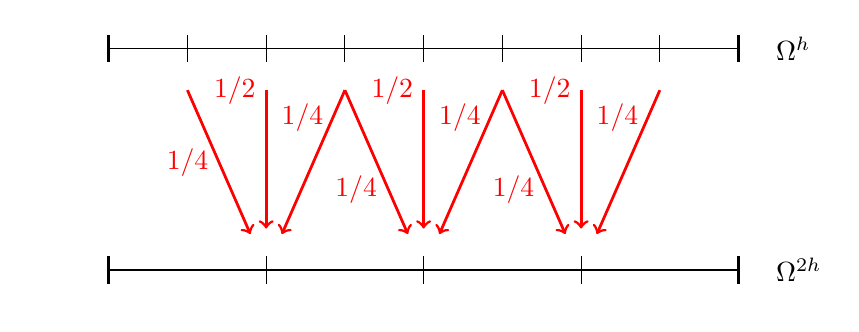
\begin{tikzpicture}
    \draw (0, 0) node[left]{\phantom{$\quad \Omega^{h}$}} -- (8, 0) node[right]{$\quad \Omega^{h}$};
    \draw[line width = 1pt] (0, .5em) -- (0, -.5em) node[below] {} ;
    \draw[line width = 1pt] (8, .5em) -- (8, -.5em) node[below] {} ;
    \foreach \x in {1, ..., 7}
        \draw[shift={(\x, 0)}] (0, .5em) -- (0, -.5em);

    \draw (0, -8em) node[right]{\phantom{$\quad \Omega^{2h}$}}-- (8, -8em) node[right]{$\quad \Omega^{2h}$};
    \draw[line width = 1pt] (0, -7.5em) -- (0, -8.5em) node[below] {} ;
    \draw[line width = 1pt] (8, -7.5em) -- (8, -8.5em) node[below] {} ;
    \foreach \x in {2, 4, 6}
        \draw[shift={(\x, 0)}] (0, -7.5em) -- (0, -8.5em);
    
    {
    \color{red}
    %% n = 1
    \draw[->, line width=1pt] 
    (1, -1.5em) 
    -- 
    (1.8, -6.7em) node[midway, left]{1/4} ;
    \draw[->, line width=1pt] 
    (2, -1.5em) node[left]{1/2} 
    -- 
    (2, -6.5em)
    ;
    \draw[->, line width=1pt] 
    (3, -1.5em) node[left, yshift=-1em, xshift=-.4em]{1/4} 
    -- 
    (2.2, -6.7em)  ;
    
    %% n = 4
    \draw[->, line width=1pt] 
    (3, -1.5em) 
    -- 
    (3.8, -6.7em) node[midway, left, yshift=-1em, xshift=.4em]{1/4} ;
    \draw[->, line width=1pt] 
    (4, -1.5em) node[left]{1/2} 
    -- 
    (4, -6.5em)
    ;
    \draw[->, line width=1pt] 
    (5, -1.5em) node[left, yshift=-1em, xshift=-.4em]{1/4} 
    -- 
    (4.2, -6.7em)  ;
    
    %% n = 6
    \draw[->, line width=1pt] 
    (5, -1.5em) 
    -- 
    (5.8, -6.7em) node[midway, left, yshift=-1em, xshift=.4em]{1/4} ;
    \draw[->, line width=1pt] 
    (6, -1.5em) node[left]{1/2} 
    -- 
    (6, -6.5em)
    ;
    \draw[->, line width=1pt] 
    (7, -1.5em) node[left, yshift=-1em, xshift=-.4em]{1/4} 
    -- 
    (6.2, -6.7em)  ;
    }
\end{tikzpicture}

\end{center}


For prolongation, we typically use a linear interpolant at the new grid points 

\begin{center}
    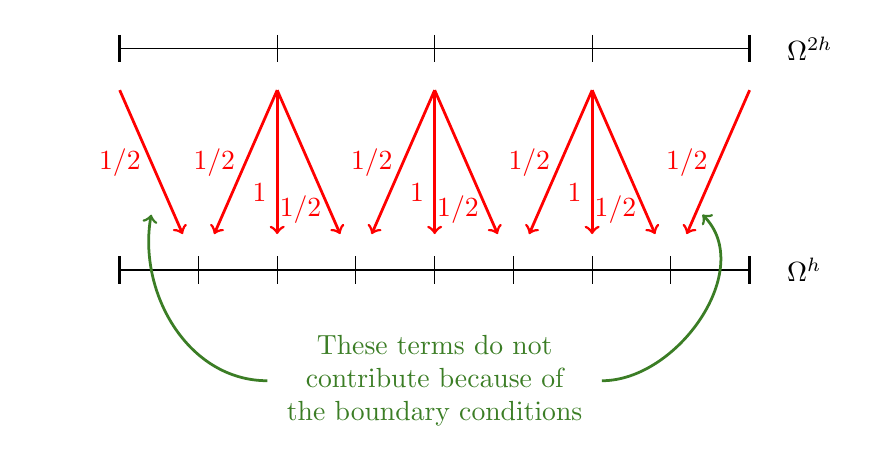
\begin{tikzpicture}
    \draw (0, -8em) node[right]{\phantom{$\quad \Omega^{h}$}}-- (8, -8em) node[right]{$\quad \Omega^{h}$};
    \draw[line width = 1pt] (0, .5em) -- (0, -.5em) node[below] {} ;
    \draw[line width = 1pt] (8, .5em) -- (8, -.5em) node[below] {} ;
    \foreach \x in {2, 4, 6}
        \draw[shift={(\x, 0)}] (0, .5em) -- (0, -.5em);

    \draw (0, 0) node[left]{\phantom{$\quad \Omega^{2h}$}} -- (8, 0) node[right]{$\quad \Omega^{2h}$};
    \draw[line width = 1pt] (0, -7.5em) -- (0, -8.5em) node[below] {} ;
    \draw[line width = 1pt] (8, -7.5em) -- (8, -8.5em) node[below] {} ;
    \foreach \x in {1, ..., 7}
        \draw[shift={(\x, 0)}] (0, -7.5em) -- (0, -8.5em);
    
    {
    \color{red}
    %% n = 1
    
    \draw[->, line width=1pt] 
    (0, -1.5em) 
    -- 
    (0.8, -6.7em) node[midway, left]{1/2} ;
    \draw[->, line width=1pt] 
    (2, -1.5em) 
    -- 
    (1.2, -6.7em)node[midway,left]{1/2} 
    ;
    \draw[->, line width=1pt] 
    (2, -1.5em)  
    -- 
    (2, -6.7em) node[left, yshift=1.5em]{1} ;
    \draw[->, line width=1pt] 
    (2, -1.5em)  
    -- 
    (2.8, -6.7em) node[left, yshift=.9em, xshift=-.3em]{1/2} ;
    
    \draw[->, line width=1pt] 
    (4, -1.5em) 
    -- 
    (3.2, -6.7em)node[midway,left]{1/2} 
    ;
    \draw[->, line width=1pt] 
    (4, -1.5em)  
    -- 
    (4, -6.7em) node[left, yshift=1.5em]{1} ;
    \draw[->, line width=1pt] 
    (4, -1.5em)  
    -- 
    (4.8, -6.7em) node[left, yshift=.9em, xshift=-.3em]{1/2} ;
    
    \draw[->, line width=1pt] 
    (6, -1.5em) 
    -- 
    (5.2, -6.7em)node[midway,left]{1/2} 
    ;
    \draw[->, line width=1pt] 
    (6, -1.5em)  
    -- 
    (6, -6.7em) node[left, yshift=1.5em]{1} ;
    \draw[->, line width=1pt] 
    (6, -1.5em)  
    -- 
    (6.8, -6.7em) node[left, yshift=.9em, xshift=-.3em]{1/2} ;
    \draw[->, line width=1pt] 
    (8, -1.5em) 
    -- 
    (7.2, -6.7em)node[midway,left]{1/2} 
    ;
    }
    {
    \color{OliveGreen}
    \node[text width=4cm,align=center] (text) at (4, -12em) {These terms do not contribute because of the boundary conditions};
    \draw[->, line width=1pt] (text.west) to[out=180, in=-100] (0.4, -6em);
    \draw[->, line width=1pt] (text.east) to[out=0, in=-45] (7.4, -6em);
    }
\end{tikzpicture}

\end{center}

We introduce the following notation
\begin{itemize}[{label={}}]
\item Smoother$(\vec{v}^{\,h}, \vec{f}^{\,h}) \rightarrow$ Apply 1 step of the
smoother (Ex.\ weighted Jacobi) to the linear system $A^h\vec{u}^{\,h}
=\vec{f}^{\,h}$ with initial guess $\vec{v}^{\,h}$

\item $\mathcal{I}_{h}^{2h} \rightarrow$ restrict a vector on grid $\Omega^h$ to a
vector on $\Omega^{2h}$

\item $\mathcal{I}_{2h}^{h} \rightarrow$ prolong a vector on grid $\Omega^{2h}$ to a
vector on $\Omega^{h}$
\end{itemize}

Therefore, our two-grid multigrid scheme is the following. Given an initial
guess of $\vec{v}^{\,h}$ of $A^h\vec{u} =\vec{f}^{\,h}$

\begin{itemize}{}
\item $\vec{v}^{\,h} = \text{Smoother}(\vec{v}^{\,h}, \vec{f}^{\,h}) \qquad k=1, \ldots, \nu_1$
\item $\vec{r}^{\,h} = \vec{f}^{\,h} - A^h\vec{v}^{\,h}$
\item $\vec{r}^{\,2h} = \mathcal{I}_{h}^{2h}\vec{r}^{\,h}$
\item Solve $A^{2h}\vec{e}^{\,2h} = \vec{r}^{\,2h} \quad$ for $\vec{e}^{\,2h}$
\item $\vec{e}^{\,h} = \mathcal{I}_{2h}^{h}\vec{e}^{\,2h}$
\item $\vec{v}^{\,h} = \vec{v}^{\,h} + \vec{e}^{\,h}$
\item $\vec{v}^{\,h} = \text{Smoother}(\vec{v}^{\,h}, \vec{f}^{\,h}) \qquad k=1, \ldots, \nu_2$
\end{itemize}

%% Lecture 12

Note that this is \underline{not} a solver, but instead is an iterative method
that takes an initial guess $\vec{v}^{\,h}$ of $A^h\vec{u} = \vec{f}^{\,h}$, and
hopefully returns a more accurate solution.

We can calculate the number of flops to apply this two-grid cycle once. The main
steps are

\begin{enumerate}[1)]
\item Apply smoother $\nu_1 + \nu_2$ times. Since A is sparse (tridiagonal),
  this costs $\bigO{(\nu_1 + \nu_2)n}$ operations. 
\item Compute the residual $\vec{r}^{\,h} = \vec{f}^{\,h} - A^h\vec{v}^{\,h}$.
  This costs $\bigO{n}$ operations.
\item Apply the restriction and prolongation operators. Each of these steps
  requires visiting each of the $n$ points once, and doing $\bigO{1}$ operations
  at each point. Therefore, prolongation and restriction cost $\bigO{n}$
  operations.
\item Solve $A^{2h}\vec{e}^{\,2h} = \vec{r}^{\,2h}$. This cost depends on how we
  solve this system. It actually doesn't even have to be solved exactly. 
  \begin{enumerate}[a)]
  \item Solve with Gaussian elimination/$LU$/$QR$/etc.\ with a cost of
    $\bigO{\left(\frac{n}{2}\right)^3} = \bigO{n^3/8}$ operations.
  \item Solve approximatly with Jacobi/SOR/Gauss-Siedell/etc.\ 
    with a cost of $\bigO{n\cdot n_{\text{iter}}}$ where the iterative method is
    applied $n_{\text{iter}}$ times. 
  \item TBD
  \end{enumerate}
\end{enumerate}

Suppose we did Gaussian elimination at the coarse grid solve. Then the cost is
\vspace{2em}
\begin{equation*}
\mathcal{O}\left( (\tikzmark{nu1}\nu_1 + \tikzmark{nu2}\nu_2 + \tikzmark{resid}1 + \tikzmark{restrict}1 + \tikzmark{prolong}1)n + \frac{n^3}{8} \right) \quad\text{operations}
\end{equation*}

{
\color{red}

\begin{tikzpicture}[overlay,remember picture]

\node (presmooth) [below of=nu1, node distance = 3 em, xshift=-1em] {pre-smoothing};
\draw [<-] (nu1)++(.25em,-.5ex) to[out=-90, in=50] (presmooth);

\node (postsmooth) [below of=nu2, node distance = 5 em] {post-smoothing};
\draw [<-] (nu2)++(.25em,-.5ex) to[out=-90, in=45] (postsmooth);

\node (comp_r) [below of=resid, node distance = 3 em, anchor=west] {Compute $\vec{r}^{\,h}$};
\draw [<-] (resid)++(.25em,-.5ex) to [out=-90, in=90] (comp_r);

\node (restI) [above of=restrict, node distance = 3 em] {$\mathcal{I}_{h}^{2h}$};
\draw [<-] (restrict)++(.25em,1em) to (restI);


\node (proI) [above of=prolong, node distance = 3 em, anchor=west] {$\mathcal{I}_{2h}^{h}$};
\draw [<-] (prolong)++(.25em,1em) to (proI);

\end{tikzpicture}
}

\vspace{2em}

However, doing Gaussian eliminations to $A^h\vec{u} = \vec{f}^{\,h}$ requires
$\bigO{n^3}$ operations. Therefore, if not too many two-grid cycles are required,
our two-grid algorithm can out perform Gaussian elimination.

\pagebreak

\subsection{Recursive Multigrid}
Regarding option c), we note that we are solving

\begin{equation*}
A^{2h}\vec{e}^{\,2h} = \vec{r}^{\,2h}
\end{equation*}

This is just another linear system, albeit a smaller one, that can be solved
with a two-grid cycle. That is we have the following algorithm that takes in an
initial guess $\vec{v}^{\,h}$ and a right hand side $\vec{f}^{\,h}$ and returns
a better solution of $A^h\vec{u} = \vec{f}^{\,h}$.

\vspace{2em}
\begin{equation*}
\tikzmark{vh}\vec{v}^{\,h} = \tikzmark{V}V(\tikzmark{vhguess}\vec{v}^{\,h}, \tikzmark{fh}\vec{f}^{\,h})
\end{equation*}

{
\color{red}

\begin{tikzpicture}[overlay,remember picture]
\node (improved) [below of=vh, node distance = 3 em, anchor=west] {improved (hopefully) solution};
\draw [<-] (vh)++(.25em,-.5ex) to [out=-90, in=180] (improved);

\node (func) [below right of=V, node distance = 2 em,anchor=west] {function};
\draw [<-] (V)++(.25em,-.5ex) to [out=-90, in=180] (func);

\node (current) [above of=V, node distance = 2 em,anchor=east] {current guess};
\draw [<-] (vhguess)++(.25em,1em) to [out=90, in=0] (current);

\node (RHS) [above of=fh, node distance = 3 em,anchor=west] {right hand side};
\draw [<-] (fh)++(.45em,1em) to [out=80, in=-90] (RHS);
\end{tikzpicture}
}
\vspace{2em}

\begin{algorithm}
    \caption{V-cycle}
    \begin{algorithmic} 
      \STATE $\vec{v}^{\,h} \enspace = \text{Smoother}(\vec{v}^{\,h}, \vec{f}^{\,h}) \qquad k=1, \ldots, \nu_1$ 
      \STATE $\vec{f}^{\,2h} = \mathcal{I}_{h}^{2h}(\vec{f}^{\,h} - A^h\vec{v}^{\,h})$

      \STATE \qquad $\vec{v}^{\,2h} = \vec{0}$ 
      \STATE \qquad $\vec{v}^{\,2h} = \text{Smoother}(\vec{v}^{\,2h}, \vec{f}^{\,2h}) \qquad k=1, \ldots, \nu_1$ 
      \STATE \qquad $\vec{f}^{\,4h} = \mathcal{I}_{2h}^{4h}(\vec{f}^{\,2h} - A^{2h}\vec{v}^{\,2h})$

      \STATE \qquad\qquad $\vec{v}^{\,4h} = \vec{0}$ 
      \STATE \qquad\qquad $\vec{v}^{\,4h} = \text{Smoother}(\vec{v}^{\,4h}, \vec{f}^{\,4h}) \qquad k=1, \ldots, \nu_1$ 
      \STATE \qquad\qquad $\vec{f}^{\,8h} = \mathcal{I}_{4h}^{8h}(\vec{f}^{\,4h} - A^{4h}\vec{v}^{\,4h})$

      \STATE \qquad\qquad\qquad $\ddots$
      \STATE \qquad\qquad\qquad\quad $\vec{v}^{\,Lh}=\left( A^{Lh} \right)^{-1}\vec{f}^{\,Lh}$
      \STATE \qquad\qquad\qquad \reflectbox{$\ddots$}

      \STATE \qquad\qquad $\vec{v}^{\,4h}  = \vec{v}^{\,4h} + \mathcal{I}_{8h}^{4h}\vec{v}^{\,8h}$
      \STATE \qquad\qquad $\vec{v}^{\,4h} = \text{Smoother}(\vec{v}^{\,4h}, \vec{f}^{\,4h}) \qquad k=1, \ldots, \nu_2$ 

      \STATE \qquad $\vec{v}^{\,2h}  = \vec{v}^{\,2h} + \mathcal{I}_{4h}^{2h}\vec{v}^{\,4h}$
      \STATE \qquad $\vec{v}^{\,2h} = \text{Smoother}(\vec{v}^{\,2h}, \vec{f}^{\,2h}) \qquad k=1, \ldots, \nu_2$ 

      \STATE $\vec{v}^{\,h}  = \vec{v}^{\,h} + \mathcal{I}_{2h}^{h}\vec{v}^{\,2h}$
      \STATE $\vec{v}^{\,h} = \text{Smoother}(\vec{v}^{\,h}, \vec{f}^{\,h}) \qquad k=1, \ldots, \nu_2$ 
    \end{algorithmic} 
\end{algorithm}
Again, this algorithm is not a solver. It returns a more accurate solution
of$A^h\vec{u} = \vec{f}^{\,h}$. We can visualize the algorithm as follows. 


\begin{center}
        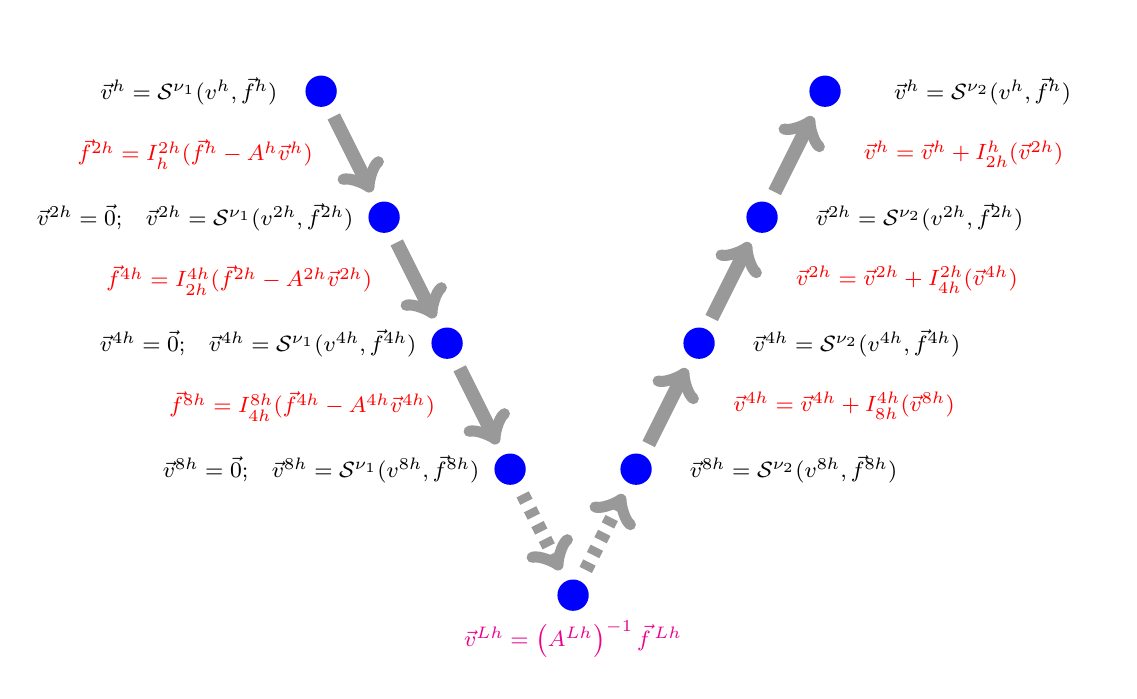
\begin{tikzpicture}[scale=0.8]
  \draw[white] (-8.5,9)--(8.5,9)--(8.5,-1.2)--(-8.5,-1.2)--cycle;
    \node[circle, fill=blue, inner sep=4pt,minimum size=2pt,line
    width=0pt] at (-4,8) {};

    \node at (-6.1,8) {\footnotesize $\vec{v}^h = 
      \mathcal{S}^{\nu_1}(v^h,\vec{f}^h)$};

    \draw[black!40,line width=5pt,->]
    (-3.8,7.6)--(-3.2,6.4);
    \node[red] at (-6.0,7.0) {\footnotesize $\vec{f}^{2h} = 
      I^{2h}_{h}(\vec{f}^h - A^h \vec{v}^h)$};
    \node[circle, fill=blue, inner sep=4pt,minimum size=2pt,line
    width=0pt] at (-3,6) {};

    \node at (-6,6) {\footnotesize $\vec{v}^{2h} = \vec{0}$;\quad $\vec{v}^{2h} = 
      \mathcal{S}^{\nu_1}(v^{2h},\vec{f}^{2h})$};

    \draw[black!40,line width=5pt,->]
    (-2.8,5.6)--(-2.2,4.4);
    \node[red] at (-5.3,5.0) {\footnotesize $\vec{f}^{4h} = 
      I^{4h}_{2h}(\vec{f}^{2h} - A^{2h} \vec{v}^{2h})$};
    \node[circle, fill=blue, inner sep=4pt,minimum size=2pt,line
    width=0pt] at (-2,4) {};

    \node at (-5,4) {\footnotesize $\vec{v}^{4h} = \vec{0}$;\quad $\vec{v}^{4h} = 
      \mathcal{S}^{\nu_1}(v^{4h},\vec{f}^{4h})$};

    \draw[black!40,line width=5pt,->]
    (-1.8,3.6)--(-1.2,2.4);
    \node[red] at (-4.3,3.0) {\footnotesize $\vec{f}^{8h} = 
      I^{8h}_{4h}(\vec{f}^{4h} - A^{4h} \vec{v}^{4h})$};
    \node[circle, fill=blue, inner sep=4pt,minimum size=2pt,line
    width=0pt] at (-1,2) {};

    \node at (-4,2) {\footnotesize $\vec{v}^{8h} = \vec{0}$;\quad $\vec{v}^{8h} = 
      \mathcal{S}^{\nu_1}(v^{8h},\vec{f}^{8h})$};

    \draw[black!40,line width=5pt,->,dashed]
    (-0.8,1.6)--(-0.2,0.4);
    \node[circle, fill=blue, inner sep=4pt,minimum size=2pt,line
    width=0pt] at (0,0) {};

    \node[magenta] at (0,-0.7) {\footnotesize $\vec{v}^{Lh} = 
      \left(A^{Lh}\right)^{-1} \vec{f}^{\,Lh}$};

    \draw[black!40,line width=5pt,->,dashed] (0.2,0.4)--(0.8,1.6);
    \node[circle, fill=blue, inner sep=4pt,minimum size=2pt,line
    width=0pt] at (1,2) {};

    \node at (3.5,2) {\footnotesize $\vec{v}^{8h} = 
      \mathcal{S}^{\nu_2}(v^{8h},\vec{f}^{8h})$};

    \draw[black!40,line width=5pt,->] (1.2,2.4)--(1.8,3.6);
    \node[red] at (4.3,3.0) {\footnotesize $\vec{v}^{4h} = 
      \vec{v}^{4h} + I^{4h}_{8h}(\vec{v}^{8h})$};
    \node[circle, fill=blue, inner sep=4pt,minimum size=2pt,line
    width=0pt] at (2,4) {};

    \node at (4.5,4) {\footnotesize $\vec{v}^{4h} = 
      \mathcal{S}^{\nu_2}(v^{4h},\vec{f}^{4h})$};

    \draw[black!40,line width=5pt,->] (2.2,4.4)--(2.8,5.6);
    \node[red] at (5.3,5.0) {\footnotesize $\vec{v}^{2h} = 
      \vec{v}^{2h} + I^{2h}_{4h}(\vec{v}^{4h})$};
    \node[circle, fill=blue, inner sep=4pt,minimum size=2pt,line
    width=0pt] at (3,6) {};

    \node at (5.5,6) {\footnotesize $\vec{v}^{2h} = 
      \mathcal{S}^{\nu_2}(v^{2h},\vec{f}^{2h})$};

    \draw[black!40,line width=5pt,->] (3.2,6.4)--(3.8,7.6);
    \node[red] at (6.2,7.0) {\footnotesize $\vec{v}^{h} = 
      \vec{v}^{h} + I^{h}_{2h}(\vec{v}^{2h})$};
    \node[circle, fill=blue, inner sep=4pt,minimum size=2pt,line
    width=0pt] at (4,8) {};

    \node at (6.5,8) {\footnotesize $\vec{v}^{h} = 
      \mathcal{S}^{\nu_2}(v^{h},\vec{f}^{h})$};

  \end{tikzpicture}

\end{center}

Because of the shape of this picture we call the algorithm $\vec{v}^{\,h}
\leftarrow V(\vec{v}^{\,h}, \vec{f}^{\,h})$ a \emph{V-cycle}

%% Lecture 13

Notice how at each level, we are simply applying another V-cycle, just with
fewer levels. Thus the algorithm can be written very compactly using recursion:

\begin{algorithm}
    \caption{V-cycle  $\vec{v}^{\,h}=V\left( \vec{v}^{\,h}, \vec{f}^{\,h} \right)$}
    \begin{algorithmic} 
      \STATE $\vec{v}^{\,h} \enspace = \text{Smoother}(\vec{v}^{\,h}, \vec{f}^{\,h}) \qquad k=1, \ldots, \nu_1$ 
      \STATE $\vec{f}^{\,2h} = \mathcal{I}_{h}^{2h}(\vec{f}^{\,h} - A^h\vec{v}^{\,h})$
      \IF {$\Omega^{\,2h}$ is the coarsest grid}
      \STATE Solve $A^{\,2h}\vec{v}^{\,2h} = \vec{f}^{\,2h}$
      \ELSE
      \STATE $\vec{v}^{\,2h} = \vec{0}$
      \STATE $\vec{v}^{\,2h} = V(\vec{v}^{\,2h}, \vec{f}^{\,2h})$
      \ENDIF
      \STATE $\vec{v}^{\,h}  = \vec{v}^{\,h} + \mathcal{I}_{2h}^{h}\vec{v}^{\,2h}$
      \STATE $\vec{v}^{\,h} = \text{Smoother}(\vec{v}^{\,h}, \vec{f}^{\,h}) \qquad k=1, \ldots, \nu_2$ 
    \end{algorithmic} 
\end{algorithm}

When applying a V-cycle with $\nu_1$ pre-smoothing and $\nu_2$ post-smoothing
steps, we call it a $V(\nu_1, \nu_2)$-cycle.

Let's estimate the number of flops required  to apply the $V(\nu_1,
\nu_2)$-cycle. The four main costs come from:

\begin{enumerate}[1)]
\item Apply the smoother at all levels
\item Compute the residual
\item Prolongation and restriction
\item Course-grid solve
\end{enumerate}


We ignore updating the solution
\begin{equation*}
\text{ie.\quad}\vec{v}^{\,h}  = \vec{v}^{\,h} + \mathcal{I}_{2h}^{h}\vec{v}^{\,2h}
\end{equation*}

we also ignore prolongation and restriction. Suppose there are $L$ levels. That
is, we apply the smoother on the grids
\begin{equation*}
\Omega^{h},
\Omega^{2h},
\Omega^{4h},
\ldots,
\Omega^{2^{L-1}h}
\end{equation*}

On grid $\Omega^{h}$, the smoother requires $\bigO{n}$ operations. 

On grid $\Omega^{2h}$, the smoother requires $\bigO{\frac{n}{2}}$ operations. 

\hspace{4cm}$\vdots$

On grid $\Omega^{2^{L-1}h}$, the smoother requires $\bigO{\frac{n}{2^{L-1}}}$ operations. 

Therefore, one smoother per level requires
\begin{align*}
  \bigO{n+\frac{n}{2} + \frac{n}{4} + \ldots + \frac{n}{2^{L-1}}}
  &= \bigO{n\left(1+\frac{1}{2} + \frac{1}{4} + \ldots + \frac{1}{2^{L-1}}\right)}\\
  &=\bigO{n \left( \frac{1-\left( \frac{1}{2}\right)^L}{1-\frac{1}{2}} \right) }\\
  &= \bigO{2n \left( 1-\frac{1}{2^L}\right)}
\end{align*}

$\Rightarrow$ The cost of pre-smoothing and post-smoothing is

\begin{align*}
\bigO{2(\nu_1+\nu_2) \left( 1-\frac{1}{2^L} \right)n } \quad \text{operations}
\end{align*}

The cost of computing all of the residuals is

\begin{align*}
\bigO{2 \left( 1-\frac{1}{2^L} \right)n } \quad \text{operations}
\end{align*}

Solving the coarse-grid equation requires no more than 

\begin{equation*}
\bigO{ \left( \frac{n}{2^{L-1}}\right)^3 }\quad \text{operations}
\end{equation*}

We would like to choose a value for $L$ so that $\frac{n}{2^{L-1}}$ is order 1.

\begin{align*}
\Rightarrow \frac{n}{2^{L-1}} &= \bigO{1}\\
  \Rightarrow n &= \bigO{2^{L-1}} \\
  \Rightarrow \log_2 n &=\bigO{L-1}\\
  \Rightarrow L &= \bigO{\log_2n}
\end{align*}
With this coice for $L$, the smoothing and residual operations cost $\bigO{n}$
flops and the 
coarse-grid solve requires $\bigO{1}$ operations.

\subsection{Multigrid Cycles}
The V-cycle recursively performs one V-cycle per level. Alternatively, we could
apply $\mu \in \mathbb{N}$ V-cycles per level. If $\mu=2$, the result is a
W-cycle. The schedule of the grids are as follows. 

\begin{center}
    \begin{tikzpicture}[scale=1.25]
\draw (0, 0) -- (-.5em, 0) node[anchor=east, yshift=.2em]{$\Omega^{\,h}$};
\foreach[count=\i] \x in {2, 4, 8}
\draw[shift={(0, -\i)}] (0, 0) -- (-.5em, 0)  node[anchor=east, yshift=.2em]{$\Omega^{\,\x h}$};

\def\dx{0.5};

\def\cycle{0, 1, 2, 3, 2, 3, 2, 1, 2, 3, 2, 3, 2, 1, 0};

\foreach[count=\step, evaluate=\step as \x using \step*\dx] \level in \cycle
    \node[circle,fill=black,inner sep=0em,minimum size=.5em] 
    (\step) at (\x, -\level) {};
    
\foreach \level [count=\step, remember=\step-1 as \prestep] in \cycle
    \ifnum\step>1  \path (\prestep) edge (\step) \fi;
    
    {\color{C3}
    \draw[thick, dashed] (3)++(-0.25, 0.25)  rectangle ++(2.5, -1.5);
    \node[yshift=-2cm] () at (5) {2 V-cycles};
    }
    
    {\color{C2}
    \draw[thick, dashed] (2)++(-0.25, 0.25)  rectangle ++(6.5, -3.3);
    \node[yshift=-4.25cm] () at (8) {2 V-cycles};
    }
\end{tikzpicture}

\end{center}

If we add another level the W-cycle would look like

\begin{center}
    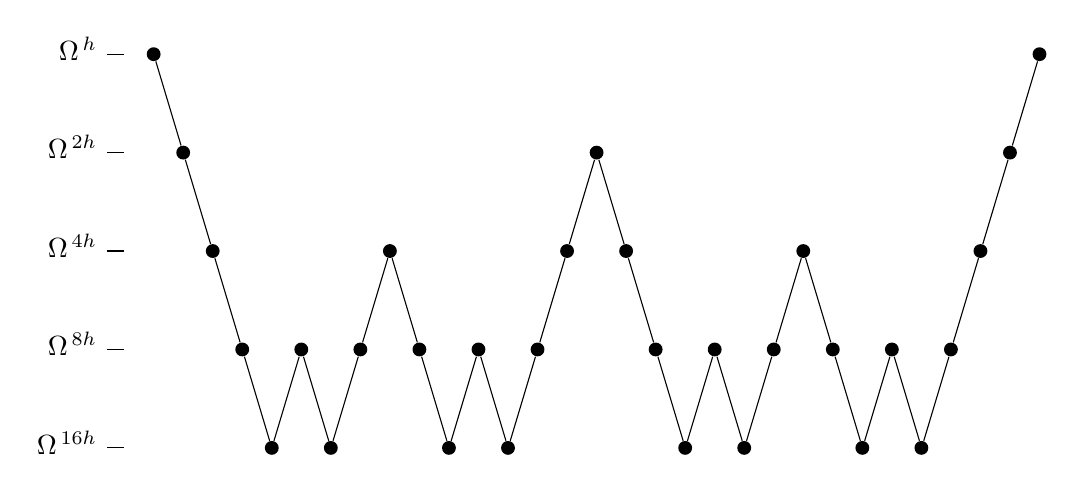
\begin{tikzpicture}[scale=1.25]
\draw (0, 0) -- (-.5em, 0) node[ anchor=east,  yshift=.2em ]{$\Omega^{\,h}$};
\foreach[count=\i] \x in {2, 4, 8, 16}
\draw[shift={(0, -\i)}] (0, 0) -- (-.5em, 0)  node[ anchor=east,  yshift=.2em]{$\Omega^{\,\x h}$};

\def\dx{0.3};

\def\cycle{
0, 1, 2, 3, 4, 3, 4, 3, 2, 3, 4, 3,4, 3, 2, 1, 2, 3, 4, 3, 4, 3, 2, 3, 4, 3, 4, 3,  2, 1, 0
};

\foreach[count=\step, evaluate=\step as \x using \step*\dx] \level in \cycle
    \node[circle,fill=black,inner sep=0em,minimum size=.5em] 
    (\step) at (\x, -\level) {};
    
\foreach \level [count=\step, remember=\step-1 as \prestep] in \cycle
    \ifnum\step>1  \path (\prestep) edge (\step) \fi;
    
\end{tikzpicture}


\end{center}

%% Lecture 14

Once you have a good recursive V-cycle code, Implementing a W-cycle is trivial.


\begin{center}
\begin{tabular}[t]{lcl}
  \underline{V-Cycle} & & \underline{W-Cycle} \\
  $\vec{v}^{\,2h} = 0$ &\textcolor{red}{Changes} & $\vec{v}^{\,2h} = 0$\\
  $\vec{v}^{\,2h} = V(\vec{v}^{\,2h}, \vec{f}^{\,2h})$ &\textcolor{red}{to}&$\vec{v}^{\,2h} = V(\vec{v}^{\,2h}, \vec{f}^{\,2h})$\\
  &&$\vec{v}^{\,2h} = V(\vec{v}^{\,2h}, \vec{f}^{\,2h})$
\end{tabular}
\end{center}

The W-cycle costs more per iterations, but it does a better job of eliminating
intermediate frequencies. This is beneficial in $\mathbb{R}^2$ and
$\mathbb{R}^3$, but in  $\mathbb{R}^1$, more times than not, you can not out
perform a V$(1, 1)$-cycle.

The final multigrid cycle we'll consider is called \emph{full multigrid} or FMG. It is
motivated by the fact that we should choose a good initial guess. We can choose
an initial guess at the coarsest grid by solving.
\begin{equation*}
\vec{u}^{\,Lh} = (A^{Lh}) \vec{f}^{\,Lh} 
\end{equation*}
However, we need to move this initial guess to the grid $\Omega^h$. We could
just prolong the whole way up but this would not be very, accurate. Instead we
prolong once, perform a V-cycle, and repeat until we're at the finest grid. We
then perform out standard V-cycle.

\hspace{-1cm} 
\begin{tikzpicture}[node distance=.3cm]
\draw (0, 0) -- (-.5em, 0) node[ anchor=east,  yshift=.2em ]{$\Omega^{\,h}$};
\foreach[count=\i] \x in {2, 4, 8, 16}
\draw[shift={(0, -\i)}] (0, 0) -- (-.5em, 0)  node[ anchor=east,  yshift=.2em]{$\Omega^{\,\x h}$};

\def\dx{0.5};

\def\cycle{
4, 3, 4, 3, 2, 3, 4, 3, 2, 1, 2, 3, 4, 3, 2, 1, 0, 1, 2, 3, 4, 3, 2, 1, 0
};

\foreach[count=\step, evaluate=\step as \x using \step*\dx] \level in \cycle
    \node[circle,fill=black,inner sep=0em,minimum size=.5em] 
    (step\step) at (\x, -\level) {};
    
\foreach \level [count=\step, remember=\step-1 as \prestep] in \cycle
    \ifnum\step>1  \path (step\prestep) edge (step\step) \fi;

{
\color{red}
\path (step1)+(0, 3mm) -- node[left] {$\mathcal{I}^{8h}_{16h}$}  (step2);
\node [below right =  4mm and -.5 of step1), anchor=west] () {Solve $A^{16h} \vec{u}^{\,16h} = \vec{f}^{\,16h}$};

\path (step2) edge[<->] node[above](){\scriptsize 1 V-cycle}(step4);
\node[above left = of step5](){$\mathcal{I}^{4h}_{8h}$} edge[->] (2.2, -2.5) ;

\path (step5) edge[<->] node[above](){\scriptsize 1 V-cycle}(step9);
\node[above left = of step10](){$\mathcal{I}^{2h}_{4h}$} edge[->] (4.65, -1.5) ;


\path (step10) edge[<->] node[above](){\scriptsize 1 V-cycle} (step16);
\node[left = of step17](){$\mathcal{I}^{h}_{2h}$} edge[->] (8.2, -.5) ;

\path (step17) edge[<->] node[above](){\scriptsize 1 V-cycle} (step25);


}


\end{tikzpicture}


Some generalizations are
\begin{enumerate}[1)]
\item Do W-cycles instead of V-cycles.
\item Do more than one V-cycle or W-cycle starting at the finest grid.  
\item Do more than 1 V-cycle or W-cycle when forming the initial guess. 
\end{enumerate}

\subsection{Multigrid in $\mathbb{R}^2$}
Multigrid is not very practical for solving
\begin{align*}
  u^{''} &= f \qquad  x\in (0, 1) \\
  u(0)&=u(1)=0
\end{align*}

with second-order centered differences. Instead, we should solve this system
with the Thomas algorithm in $\bigO{n}$ operation. However, in $\mathbb{R}^2$ or
higher, we are solving 

\begin{align*}
  \Delta u &= \frac{\partial^2u}{\partial x^2}  + \frac{\partial^2u}{\partial y^2}  = f(x,y) & (x, y)\in (0, 1)\\
  u&=0& (x, y)\in \partial(0,1)
\end{align*}

After discretizing this problem with centered differenece, multigrid becomes
much more powerful.

The linear system to solve

\begin{equation*}
  f_{i, j} = \frac{
    U_{i+1, j} + U_{i-1, j} + U_{i, j+1} + U_{i, j-1} - 4U_{i, j}
  }{h^2} \qquad\substack{i=1, \ldots, n \\ j=1, \ldots, n}
\end{equation*}
Where $\Delta x=\Delta y=h=\frac{1}{n+1}$ and $U_{i,j}\approx u(x_i, y_j)$ with $x_i=ih,\,y_j=jh$

\begin{center}
    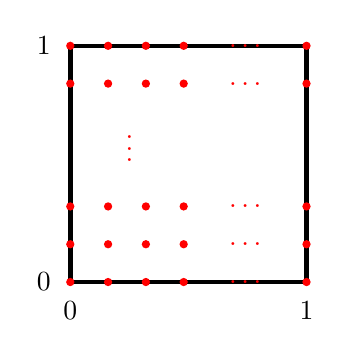
\begin{tikzpicture}[scale=3]

\draw[ultra thick] (0, 0) rectangle (1, 1);

\node[label=left:0, label=below:0] at (0, 0){};
\node[label=left:1] at (0, 1){};
\node[label=below:1] at (1, 0){};

\foreach \x in {0, 0.16, ..., 0.5}
\foreach \y in {0, 0.16, ..., 0.4}
\node[fill, circle, inner sep = 0pt, minimum size=3pt, red] at (\x, \y) {};

\foreach \y in {0, 0.16, ..., 0.4}
\node[fill, circle, inner sep = 0pt, minimum size=3pt, red] at (1, \y) {};

\foreach \y in {1, 0.84, ..., 0.77}
\node[fill, circle, inner sep = 0pt, minimum size=3pt, red] at (1, \y) {};

\foreach \y in {0, 0.16, ..., 0.4}
\node[inner sep = 0pt, minimum size=3pt, red] at (.75, \y) {\ldots};

\foreach \y in {1, 0.84, ..., 0.77}
\node[inner sep = 0pt, minimum size=3pt, red] at (.75, \y) {\ldots};

\foreach \y in {1, 0.84, ..., 0.77}
\foreach \x in {0, 0.16, ..., 0.5}
\node[fill, circle, inner sep = 0pt, minimum size=3pt, red] at (\x, \y) {};

\node[red] at (.25, .6) {$\vdots$};
\end{tikzpicture}

\end{center}
Note that we have removed the boundary points from the linear system. We use a
lexicographic ordering of $U_{i, j}$

\begin{equation*}
\frac{1}{h^2}
\begin{tikzpicture}[baseline=(current bounding box.center)]
    \matrix (m) [bmatrix]{
    -4 & 1 & & \bigzero&     1& & &
    \\
    1  & -4 & 1&&    &1&&\bigzero
    \\
    &&&           &&&
    \\
    \bigzero && &1 &\bigzero&
    \\
    && 1 & -4 &&&&1
    \\
    1 &  &\bigzero  &   & -4 &  1 &    &\bigzero    &   1 &   &      && & 
    \\
      & 1&  &   &  1 & -4 & 1  &    &     & 1 &      && \bigzero& 
      \\
      &  &  &   &    &    &    &    &     &   &      && & 
      \\
      \bigzero &  &  &   & \bigzero   &    &    &  1 &     &\bigzero   &      && & 
      \\
      &  &  & 1 &    &    & 1  & -4 &     &   &      && & 1 &&&&&&
      \\ \\ \\ \\ \\ \\ \\ \\ \\ \\ \\ \\ \\ \\ \\ \\ \\ \\ \\ \\ 
    } ;
    % First Row
    \draw[dots] (m-2-2) -- (m-5-4);
    
    \draw[dots] (m-2-3) -- (m-4-4);
    \draw[dots] (m-2-1) -- (m-5-3);
    \draw[dots] (m-2-6) -- (m-5-8);
    % Second Row
    \draw[dots] (m-7-2) -- (m-10-4);
    
    \draw[dots] (m-7-5) -- (m-10-7);
    \draw[dots] (m-7-6) -- (m-10-8);
    \draw[dots] (m-7-7) -- (m-9-8);
    
    \draw[dots] (m-7-10) -- (m-10-14);
    
    \coordinate [above right = 0.3 of m-1-4] (l1);
    \draw[dashed, red, thick] (l1) -- +(0, -8.6);
        
    \coordinate [above right = 0.3 of m-1-8] (l1);
    \draw[dashed, red, thick] (l1) -- +(0, -8.6);
    
    \draw[dashed, red, thick] (l1)++(1.9, 0)-- +(0, -8.6);


    \coordinate [above left = .9mm of m-6-1] (l1);
    \draw[dashed, red, thick] (l1) -- +(8.3, 0);

    \draw[dashed, red, thick] (l1)++(0, -2.2) -- +(8.3, 0);
    \draw[dashed, red, thick] (l1)++(0, -4.2) -- +(8.3, 0);
    
  \end{tikzpicture}
 \begin{bmatrix} 
 U_{11} \\
 U_{21} \\
 \vdots \\
 U_{n1} \\
 U_{12} \\
 U_{22} \\
 \vdots \\
 U_{n2} \\
 U_{1n} \\
 U_{2n} \\
 \vdots \\
 U_{nn} \\
 \end{bmatrix} 
 =
 \begin{bmatrix} 
 f_{11} \\
 f_{21} \\
 \vdots \\
 f_{n1} \\
 f_{12} \\
 f_{22} \\
 \vdots \\
 f_{n2} \\
 f_{1n} \\
 f_{2n} \\
 \vdots \\
 f_{nn} \\
 \end{bmatrix} 
\end{equation*}

If we define 
\begin{equation*}
  T = 
\begin{tikzpicture}[baseline=(current bounding box.center)]
    \matrix (m) [bmatrix]{
      -4 & 1 &&&&\bigzero\\
      1 & -4 & 1&&&\\
               &&&&&\\
               &&&&&\\
               \bigzero&&&&&1\\
               &&&&1&-4\\
    } ;
    \draw[dots] (m-2-2) -- (m-6-6);
    \draw[dots] (m-2-1) -- (m-6-5);
    \draw[dots] (m-2-3) -- (m-5-6);
  \end{tikzpicture}
  \in \mathbb{R}^{n \times n}
  \qquad
  I = 
\begin{tikzpicture}[baseline=(current bounding box.center)]
    \matrix (m) [bmatrix]{
      1 & & & & & \bigzero\\
        & & & & & \\
        & & & & & \\
        & & & & & \\
        \bigzero& & & & & \\
        & & & & & 1\\
    } ;
    \draw[dots] (m-1-1) -- (m-6-6);
  \end{tikzpicture}
  \in \mathbb{R}^{n \times n}
\end{equation*}

then

\begin{equation*}
  A = \frac{1}{h^2}
\begin{tikzpicture}[baseline=(current bounding box.center)]
    \matrix (m) [bmatrix]{
      T & I &   &   & &   &   & \\
      I & T & I &   & &   &   \bigzero& \\
        & I & T & I & &   &   & \\
        &   &   &   & &   &   & \\
        &   &   &   & &   &   & \\
        &   &   &   & &   &   & \\
       & \bigzero   &   &   & & I & T & I\\
        &   &   &   & &   & I &T \\
    } ;
    \draw[dots] (m-3-3) -- (m-7-7);
    \draw[dots] (m-3-2) -- (m-7-6);
    \draw[dots] (m-3-4) -- (m-7-8);
  \end{tikzpicture}
\end{equation*}

%% Lecture 15
We are trying to solve

\begin{equation*}
  \frac{1}{h^2}\left(
    U_{i+1, j} + U_{i-1, j} + U_{i, j+1} + U_{i, j-1} - 4U_{i, j}
  \right)
   = f_{i,j}
\end{equation*}

The Jacobi iteration is

\begin{equation*}
    U_{i, j}^{n+1} =
    \frac{1}{4}\left(
    U_{i+1, j}^{n} + U_{i-1, j}^{n} + U_{i, j+1}^{n} + U_{i, j-1}^{n} -  h^2 f_{i,j}
      \right)
\end{equation*}

The weighted Jacobi is

\begin{equation*}
    U_{i, j}^{n+1} =
    \frac{\omega}{4}\left(
    U_{i+1, j}^{n} + U_{i-1, j}^{n} + U_{i, j+1}^{n} + U_{i, j-1}^{n} -  h^2 f_{i,j}
      \right) + (1-\omega)U_{i, j}^{n}
\end{equation*}

Using a similar argument as we did in $\mathbb{R}^1$, the optimal choice for
$\omega$ is $\omega=4/5$.


In addition to a smoother, we require a prolongation and restriction operators.

\begin{center}
    \begin{tikzpicture}[scale=1,
little label/.style={
xshift=-4mm, yshift=4mm,
color=C2
}
]
\begin{scope}
\draw[ultra thick] (0, 0) grid (4, 4);
\foreach \x in {1, 2, 3}
\foreach \y in {1, 2, 3}
\node[circle, red, fill] (n-\x-\y) at (\x, \y) {};

\node[draw=black,circle, ultra thick] () at (n-2-2) {};

\node[above = of n-2-3] () {Restriction};

\node[little label] at (n-1-3){$\frac{1}{16}$};
\node[little label] at (n-2-3){$\frac{1}{8}$};
\node[little label] at (n-3-3){$\frac{1}{16}$};

\node[little label] at (n-1-2){$\frac{1}{8}$};
\node[little label, ] at (n-2-2){$\frac{1}{4}$};
\node[little label] at (n-3-2){$\frac{1}{8}$};

\node[little label] at (n-1-1){$\frac{1}{16}$};
\node[little label] at (n-2-1){$\frac{1}{8}$};
\node[little label] at (n-3-1){$\frac{1}{16}$};
\node[below = of n-2-1] () {Full Weighting};
\end{scope}

\begin{scope}[xshift=6cm]
\draw[ultra thick] (0, 0) grid (4, 4);
\foreach \x in {1, 2, 3}
\foreach \y in {1, 2, 3}
\node[circle, red, fill] (n-\x-\y) at (\x, \y) {};
\node[above = of n-2-3] () {Prolongation};
\node[little label] at (n-1-3){$\frac{1}{4}$};
\node[little label, xshift=8mm] at (n-2-3){$\frac{1}{4}$};
\node[little label, xshift=8mm, yshift=-8mm] at (n-2-2){$\frac{1}{4}$};
\node[little label, yshift=-8mm] at (n-1-2){$\frac{1}{4}$};


\draw[red,thick, dashed] (1.5cm, 0) -- (1.5cm, 4cm);
\draw[red,thick, dashed] (0cm, 2.5cm) -- (4cm, 2.5cm);
\node[draw=black, fill=red,circle, ultra thick] () at (1.5cm, 2.5cm) {};

\node [fill=red, circle, draw=black, ultra thick] at (3cm , 1.5cm) {};
\node[little label, xshift=8mm, yshift=-8mm] at (n-3-1){$\frac{1}{2}$};
\node[little label, xshift=8mm, yshift=-8mm] at (n-3-2){$\frac{1}{2}$};

\node[below=of n-2-1](){Bilinear interpolation};
\end{scope}

\end{tikzpicture}

\end{center}
